
\section{Trapped Ion Quantum Computing} \label{sec:Trapped}
In this section we provide an introduction to the implementation details of trapped ion quantum computers (**once done possibly elaborate what exactly we covered).
The qubits in a trapped ion system are represented by individual trapped ions, as would have been seen in a quantum mechanics class, electrons bound in atoms can occupy a certain number of possible quantum states, here 2 of these level are chosen and used as the \kz and \ko states.
Though it isn't quite as simple as that, for quantum computing we must have a way of entangling these 2 states.
To achieve that, the qubits are trapped in the same trap (this will be explained further later on) and their motion within it is coupled as a quantum system through which entanglement is achieved.
Finally for qubit manipulation, lasers are used to excite and cool down the electrons and the ions themselves.

\subsection{Ion Trapping and the Paul Trap}
Ion trapping is an extensive field of expertise used for many purposes across physics and other sciences, it is an essential component of many experiments that try to manipulate individual particles, molecules or so on.
For a brief sketch of what this involves, these experiments must be done in vacuum (otherwise there would be too many other atoms around) and rely on complex electric and magnetic fields to manipulate the motion of charged atoms.
For quantum computing we are interested in trapping individual ions in a stable way, and while we want to trap multiple of them (currently about 5-100 has been achieved !43) it is important that we can tell them apart (as opposed to trapping them in bunches as is often done).

There are currently 2 dominant suitable ion trap designs, the Penning trap which uses a combination of magnetic and electric fields, and the Paul trap (Also known as Quadrupole or Radio-Frequency-Quadrupole ion irap) which uses time varying electric fields.
Penning traps are able to hold larger amounts of ions and more stably (300 ion crystals have been achieved !46), however the motion of the ions themselves is much more complicated and leads to qubit manipulation being harder to perform.
Because of that Paul traps are more commonly used for quantum computers and due to the scope of this report we will mainly focus on them.

\subsubsection{Simple Paul Trap}
Paul trap designs use time varying fields as it is not possible to confine an ion in 3D space with only static fields.
The simplest Paul trap design is composed of 4 conducting rods run in parallel to create a quadrupole electric field in the middle, \cref{fig:ITQC_RFQ_Flour} showcases a simple demo version.
Then have each of the diagonally opposite rods connected at the same voltage and have these 2 voltages be some periodic function (usually a sine or a square wave at approximatelly raio frequencies, hence the name) in antiphase, so that if at some time one is set to positive voltage, the other should be at negative voltage.
This results in a net effect of trapping a charged particle (within some range of mass to charge ratios, this setup can be used as a mass filter) along the axis of the quadrupole, why exactly this is so is well explained in (**add a source here).
Finally, for trapping along the last axis a static electric field is used, this can be achieved by for example 2 more rod segments along the quadrupole axis at either end of the whole setup, both at some positive voltage, resulting in a potential well along the axis.

\begin{figure}[h]
    \centering
    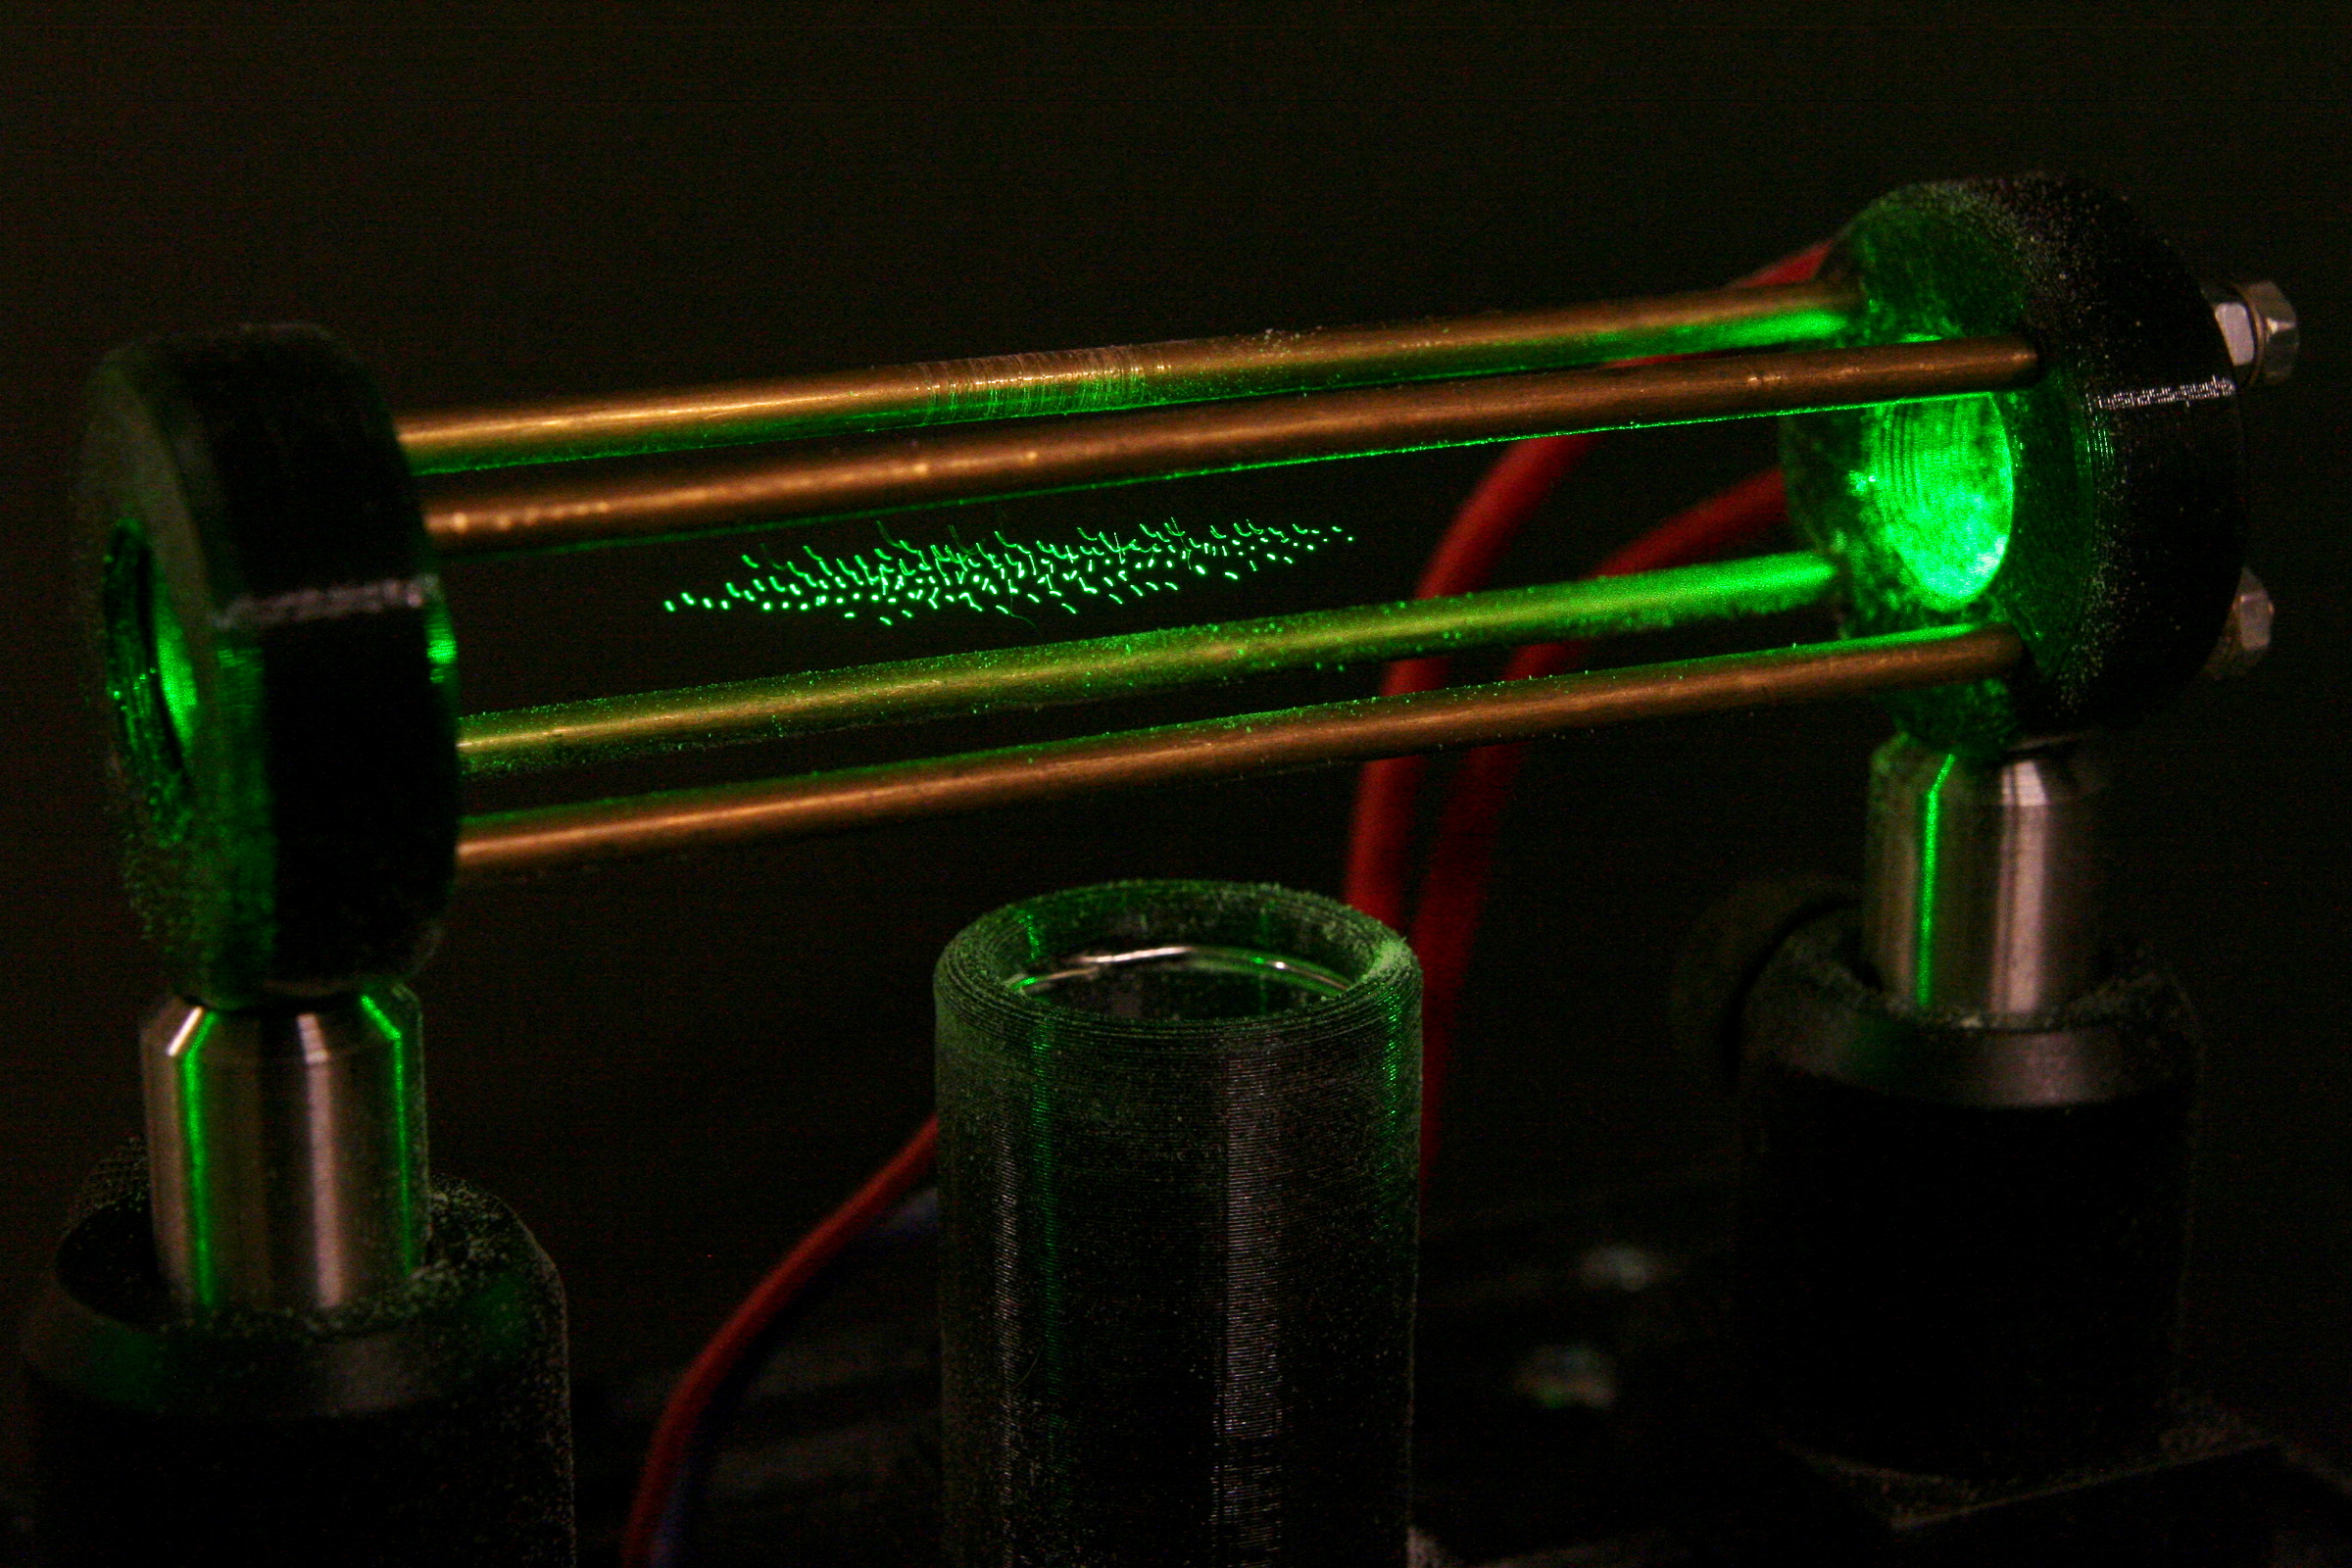
\includegraphics[width=0.9\textwidth]{images/ITQC_RFQ_Flour.jpg}
    \caption{Charged flour grains trapped in a simple Paul trap, the mentioned 4 parallel rods are visible and the electrodes creating the potential well are in the end caps.(**cite Pavelka, found on wikipedia)}\label{fig:ITQC_RFQ_Flour}
\end{figure}

\subsubsection{Notes on Other Paul Trap Designs}
Firstly, the aforementioned simple Paul trap was a linear Paul trap, in these types of Paul traps the ion's motion is confined in 2 dimensions by an RF quadrupole and the last is taken care of using a linear static potential, this is the type of trap on which we will focus.
There are also point Paul traps, which utilise oscillating RF fields for trapping in all 3 dimensions, these are also used for quantum computing, however when multiple ions are trapped together, which we need for entanglement, their motion is more complex.

Finally, there are also many different geometries for linear Paul traps, all of them result in the same ion motion along an axis, though differ greatly in design.



% There are many different ways of constructing a Paul trap, different electrode geometries give different benefits and downsides.

% For quantum computing we are mainly interested to trap individual ions in a predictable and stable way, there are 2 main types of ions traps that are used, the Penning tr
